\subsection{Text Analysis}

\subsubsection{Finding A Story}

To work on the sentiment analysis, we started working on text initially before we had enough harvested tweets. The plan was to harvest tweets predominantly from Victoria. So, based on that, we went through datasets in AURIN to come up with a story that was based on Victoria. Since, the project revolved around working with sins in tweets/text, the first thing we thought about was correlating it with a dataset for crime. One dataset that we found intriguing was LGA perception of safety – walking alone during night. We wanted to check if places where there are more tweets showcasing wrath correlated with people feeling unsafe to walk there. Based on this concept, we started to classify tweets on the sin wrath.

\subsubsection{Building A Classifier}

Since, tweets are restricted to a small set of characters that is 140 words; the texts in it are short. Due to this limitation, text in tweets is very expressive. However, this boundary may cause people to not write texts in a grammatically correct way. So, based on this assumption, we opted to focus on words in texts rather the entire text to classify it to a sin and tried solving the problem by populating a lexical resource with words that denoted the wrath. 

{\bf Preprocessing the text}


The first step we took was to remove stop words from the text. Stop words can be defined as those words that are common in texts and aren’t helpful in determining the underlying meaning of the text. The second step was to revert back words in a text to lemma. Lemma can be defined as the root word of the specific word. For instance, words such as am, are, is can be reverted back to keyword be. In our case, we could convert back annoyance, annoyed, etc. to annoy. This will help us in keyword matching. The final step is matching the words in text with text to words that give a sense of wrath and classify the text based on it. 

\begin{figure}[H]
    \centering
    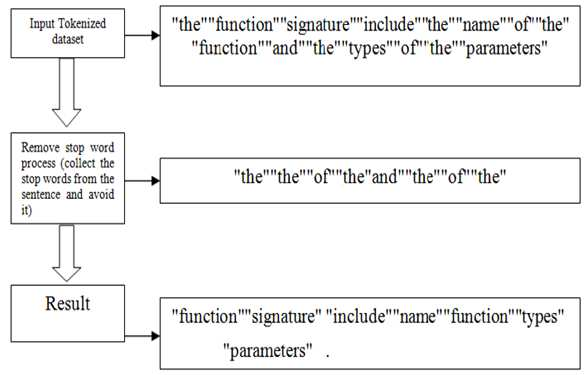
\includegraphics[width=8cm,keepaspectratio=true]{images/deployment/stop_words.png}
    \caption{Removing stop-words}
    \label{fig:stop-words-removal}
\end{figure}


{\bf Challenge 1: N-Gram Consideration}

To perform the classification, we had to take a few things in consideration. Although we can just classify text based on a single gram, but there are problems that can occur based on this. For instance, we can classify a text “I am angry today” into wrath based on the keyword anger but than this approach fails in classifying “I am not angry anymore”. Thus it is important that we don’t focus on a simple gram to perform classification. 

\vbox to 0.2cm{}
{\bf Populating the keywords for Key Word Matching}

We began with having lists for words that are synonyms and antonyms to the word wrath. A few approaches were taken into consideration to populate the list with synonyms and antonyms but we eventually decided to populate it by handpicking the synonyms. For instance, to populate synonym list we began by using a root word – wrath. By using this root word, we populated our resources with synonyms of the root word. We then populated the resource with each of the synonyms of the new word added to the resource. After certain iterations, we realized that the words that were added to the resource weren’t similar in meaning to our root word. We even tried to use WordNet along with similarity metric to limit the synonyms but the words in the list still weren’t convenient for keyword matching. 

Once the list of synonyms and antonyms were populated, lists with words that may increase the value of the words ahead of it or decrease the value of the words ahead of it. For instance “very angry” and “less angry” are examples of increase and decrease grams ahead of the word angry. Also, another list of words that inverse the meaning of the word is reversed i.e. 'not', 'non', and 'lack of' was formed. So, all these five lists were taken into consideration to give a wrath score to a text. If the wrath score of the text is above threshold, the texts were classified as denoting wrath sentiment. 


 
